\documentclass[sigconf]{acmart}

% include preamble:
%%%%%%%%%%%%%%%%%%%%%%%%%%%%%%%%%%%%%%%%%%%%%%%%%%%%%%%%%%%%%%%%%%%%%%%%%%%%%%%
% preamble for the BBOB ACM-compliant LaTeX templates                         %
%                                                                             %
% copyright 2009--2023 the BBOBies                                            %
% (under BSD licence, see https://github.com/numbbo/coco/blob/master/LICENSE) %
%%%%%%%%%%%%%%%%%%%%%%%%%%%%%%%%%%%%%%%%%%%%%%%%%%%%%%%%%%%%%%%%%%%%%%%%%%%%%%%

% to be updated from year to year:
\titlenote{Submission deadline: to be announced (likely late March/early April.}
\newcommand{\version}{2.6}


% Packages
\usepackage{booktabs} % For formal tables
\usepackage{graphicx}
\usepackage{rotating}
\usepackage{tabularx}
\usepackage{xspace}  % automatic white space after macros
\usepackage{xstring} % for string operations
\usepackage{wasysym} % Table legend with symbols input from post-processing
\usepackage{MnSymbol} % Table legend with symbols input from post-processing
\usepackage{float}
%\usepackage[dvipsnames]{xcolor}
%\usepackage[colorlinks=true, linkcolor=blue]{hyperref} % make COCO papers clickable
\usepackage{ifthen}
\usepackage{xcolor}



% define some COCO/dvipsnames colors because
% ACM style does not allow to use them directly
\definecolor{Gray}{gray}{0.6}
\definecolor{NavyBlue}{rgb}{0.0, 0.0, 0.5}
\definecolor{Magenta}{rgb}{1.0, 0.0, 1.0}
\definecolor{Black}{rgb}{0.0, 0.0, 0.0}
\definecolor{Green}{rgb}{0.0, 1.0, 0.0}
%\definecolor{NavyBlue}{HTML}{000080}
%\definecolor{Magenta}{HTML}{FF00FF}
%\definecolor{Orange}{HTML}{FFA500}
%\definecolor{CornflowerBlue}{HTML}{6495ED}
%\definecolor{YellowGreen}{HTML}{9ACD32}
%\definecolor{Gray}{HTML}{BEBEBE}
%\definecolor{Yellow}{HTML}{FFFF00}
%\definecolor{GreenYellow}{HTML}{ADFF2F}
%\definecolor{ForestGreen}{HTML}{228B22}
%\definecolor{Lavender}{HTML}{FFC0CB}
%\definecolor{SkyBlue}{HTML}{87CEEB}
%\definecolor{NavyBlue}{HTML}{000080}
%\definecolor{Goldenrod}{HTML}{DDF700}
%\definecolor{VioletRed}{HTML}{D02090}
%\definecolor{CornflowerBlue}{HTML}{6495ED}
%\definecolor{LimeGreen}{HTML}{32CD32}

% COCO LaTeX commands:
\newcommand{\includeperfprof}[1]{% include and annotate at the side
  \input{\bbobdatapath\algsfolder #1}%
  \includegraphics[height=0.24\textheight]{#1}%
  %\raisebox{.12\textheight}{
	%\parbox[b][.24\textheight]{.0868\textwidth}{\begin{scriptsize}
  %  \perfprofsidepanel % this is "\algaperfprof \vfill \algbperfprof \vfill" etc
  %\end{scriptsize}}
	%}
}
\newcommand{\rot}[2][2.5]{
  \hspace*{-3.5\baselineskip}%
  \begin{rotate}{90}\hspace{#1em}#2
  \end{rotate}}
\newcommand{\DIM}{\ensuremath{\mathrm{DIM}}}
\newcommand{\ERT}{\ensuremath{\mathrm{ERT}}}
\newcommand{\FEvals}{\ensuremath{\mathrm{FEvals}}}
\newcommand{\nruns}{\ensuremath{\mathrm{Nruns}}}
\newcommand{\Dfb}{\ensuremath{\Delta f_{\mathrm{best}}}}
\newcommand{\Df}{\ensuremath{\Delta f}}
\newcommand{\Dfg}{\ensuremath{\Delta \tau}}
\newcommand{\nbFEs}{\ensuremath{\mathrm{\#FEs}}}
\newcommand{\fopt}{\ensuremath{f_\mathrm{opt}}}
\newcommand{\ftarget}{\ensuremath{f_\mathrm{t}}}
\newcommand{\fgtarget}{\ensuremath{\tau_\mathrm{t}}}
\newcommand{\Itarget}{\ensuremath{I_\mathrm{target}}}
\newcommand{\CrE}{\ensuremath{\mathrm{CrE}}}
\newcommand{\change}[1]{{\color{red} #1}}
\newcommand{\TODO}[1]{{\color{orange} !!! #1 !!!}}
\newcommand{\bbob}{{\ttfamily bbob}\xspace}
\newcommand{\bbobnoisy}{{\ttfamily bbob-noisy}\xspace}
\newcommand{\bbobbiobj}{{\ttfamily bbob-biobj}\xspace}
\newcommand{\bbobls}{{\ttfamily bbob-largescale}\xspace}
\newcommand{\bbobmixint}{{\ttfamily bbob-mixint}\xspace}
\newcommand{\bbobcons}{{\ttfamily bbob-constrained}\xspace}
\newcommand{\DI}{\ensuremath{\Delta I_{\mathrm{HV}}^{\mathrm{COCO}}}}
\newcommand{\hvref}{\ensuremath{I_\mathrm{ref}}}


\usepackage{xcolor}
\usepackage{colortbl}
\usepackage{booktabs}
%It sets your colour line and then sets back to default (black)
\definecolor{bbobblue}{HTML}{7f7fff}
\definecolor{bbobgreen}{HTML}{7fbf7f}
\newcommand{\blueline}{\arrayrulecolor{bbobblue}\specialrule{0.15em}{0em}{0em}\arrayrulecolor{black}}
\newcommand{\greenline}{\arrayrulecolor{bbobgreen}\specialrule{0.15em}{0em}{0em}\arrayrulecolor{black}}


%%%%%%%%%%%%%%%%%%%%%%   END OF PREAMBLE   %%%%%%%%%%%%%%%%%%%%%%%%%%%%%%%%%%%%


% Copyright
%\setcopyright{none}
%\setcopyright{acmcopyright}
%\setcopyright{acmlicensed}
\setcopyright{rightsretained}
%\setcopyright{usgov}
%\setcopyright{usgovmixed}
%\setcopyright{cagov}
%\setcopyright{cagovmixed}


%%%%%%%%%%%%%%%%%%%%%%%%%%%%%%%%%%%%%%%%%%%%%%%%%%%%%


% DOI
\acmDOI{10.1145/nnnnnnn.nnnnnnn} % To be updated after completing copyright process

% ISBN
\acmISBN{978-x-xxxx-xxxx-x/YY/MM} % To be updated after completing copyright process

%Conference
\acmConference[GECCO '23]{The Genetic and Evolutionary Computation Conference 2023}{July 15--19, 2023}{Lisbon, Portugal}
\acmYear{2023}
\copyrightyear{2023}

\acmPrice{15.00}






%%%%%%%%%%%%%%%%%%%%%%   END OF PREAMBLE   %%%%%%%%%%%%%%%%%%%%%%%%%%%%%%%%%%%%


%%%%%%%%%%%%%%%%%%%%%%%%%%%%%%%%%%%%%%%%%%%%%%%%%%%%%%%%%%%%%%%%%%%%%%%%%%%%%%%
%%%%%%%%% TO BE EDITED %%%%%%%%%%%%%%%%%%%%%%%%%%%%%%%%%%%%%%%%%%%%%%%%%%%%%%%%
%%%%%%%%%%%%%%%%%%%%%%%%%%%%%%%%%%%%%%%%%%%%%%%%%%%%%%%%%%%%%%%%%%%%%%%%%%%%%%%

% Algorithm names as they appear in the tables, uncomment and adapt if necessary
% \newcommand{\algAtables}{ALGO1}  % first argument in the post-processing
% \newcommand{\algBtables}{ALGO2}  % second argument in the post-processing
% \newcommand{\algCtables}{ALGO3}  % third argument in the post-processing
% \newcommand{\algDtables}{ALGO4}  % forth argument in the post-processing
% ...
% location of pictures files
\newcommand{\bbobdatapath}{ppdata/} % change default output folder of COCO if desired


%%%%%%%%%%%%%%%%%%%%%%%%%%%%%%%%%%%%%%%%%%%%%%%%%%%%%%%%%%%%%%%%%%%%%%%%%%%%%%%
% read in data and deal with the different number of algorithms:
\input{\bbobdatapath cocopp_commands.tex}

\ifthenelse{\equal{\numofalgs}{1}}{
   \graphicspath{{\bbobdatapath\algfolder}}}{
	 \graphicspath{{\bbobdatapath\algsfolder}}
}

\ifthenelse{\isundefined{\algorithmA}}{\newcommand{\algorithmA}{\algname}}{}
%\ifthenelse{\isundefined{\algorithmA}{\newcommand{\algorithmA}{\change{MY-ALGORITHM-NAME}}}{}  % better use the previous line?
%%



%%%%%%%%%%%%%%%%%%%%%%%%%%%%%%%%%%%%%%%%%%%%%%%%%%%%%%%%%%%%%%%%%%%%%%%%%%%%%%%
%%%%%%%%%%%%%%%%%%%%%%%%%%%%%%%%%%%%%%%%%%%%%%%%%%%%%%%%%%%%%%%%%%%%%%%%%%%%%%%
%%%%%%%%%%%%%%%%%%%%%%%%%%%%%%%%%%%%%%%%%%%%%%%%%%%%%%%%%%%%%%%%%%%%%%%%%%%%%%%

\begin{document}


\title{Black-Box Optimization Benchmarking Template for the Comparison of Algorithms on the \bbobcons Testbed}
\renewcommand{\shorttitle}{Template to Compare Algorithms on the \bbobcons Testbed}
\subtitle{Draft version}



\author{Firstname Lastname}
%\authornote{tba if needed}
%\orcid{1234-5678-9012}
%\affiliation{%
%  \institution{Institute for Clarity in Documentation}
%  \streetaddress{P.O. Box 1212}
%  \city{Dublin} 
%  \state{Ohio} 
%  \postcode{43017-6221}
%}
%\email{trovato@corporation.com}
%
%\author{G.K.M. Tobin}
%\authornote{The secretary disavows any knowledge of this author's actions.}
%\affiliation{%
%  \institution{Institute for Clarity in Documentation}
%  \streetaddress{P.O. Box 1212}
%  \city{Dublin} 
%  \state{Ohio} 
%  \postcode{43017-6221}
%}
%\email{webmaster@marysville-ohio.com}
%
%\author{Lars Th{\o}rv{\"a}ld}
%\authornote{This author is the
%  one who did all the really hard work.}
%\affiliation{%
%  \institution{The Th{\o}rv{\"a}ld Group}
%  \streetaddress{1 Th{\o}rv{\"a}ld Circle}
%  \city{Hekla} 
%  \country{Iceland}}
%\email{larst@affiliation.org}
%
%\author{Lawrence P. Leipuner}
%\affiliation{
%  \institution{Brookhaven Laboratories}
%  \streetaddress{P.O. Box 5000}}
%\email{lleipuner@researchlabs.org}
%
%\author{Sean Fogarty}
%\affiliation{%
%  \institution{NASA Ames Research Center}
%  \city{Moffett Field}
%  \state{California} 
%  \postcode{94035}}
%\email{fogartys@amesres.org}
%
%\author{Charles Palmer}
%\affiliation{%
%  \institution{Palmer Research Laboratories}
%  \streetaddress{8600 Datapoint Drive}
%  \city{San Antonio}
%  \state{Texas} 
%  \postcode{78229}}
%\email{cpalmer@prl.com}
%
%\author{John Smith}
%\affiliation{\institution{The Th{\o}rv{\"a}ld Group}}
%\email{jsmith@affiliation.org}
%
%\author{Julius P.~Kumquat}
%\affiliation{\institution{The Kumquat Consortium}}
%\email{jpkumquat@consortium.net}

% The default list of authors is too long for headers}
\renewcommand{\shortauthors}{Firstname Lastname et. al.}



\begin{abstract}
to be written
\end{abstract}


%
% The code below should be generated by the tool at
% http://dl.acm.org/ccs.cfm
% Please copy and paste the code instead of the example below. 
%
 \begin{CCSXML}
<ccs2012>
<concept>
<concept_id>10010147.10010178.10010205.10010208</concept_id>
<concept_desc>Computing methodologies~Continuous space search</concept_desc>
<concept_significance>500</concept_significance>
</concept>
</ccs2012>
\end{CCSXML}

\ccsdesc[500]{Computing methodologies~Continuous space search}


% We no longer use \terms command
%\terms{Algorithms}

% Complete with anything that is needed
\keywords{Benchmarking, Black-box optimization, constrained optimization}

\maketitle


% \section{Introduction}
%
% \section{Algorithm Presentation}
%
% \section{Experimental Procedure}
%

%%%%%%%%%%%%%%%%%%%%%%%%%%%%%%%%%%%%%%%%%%%%%%%%%%%%%%%%%%%%%%%%%%%%%%%%%%%%%%%
\section{CPU Timing}
%%%%%%%%%%%%%%%%%%%%%%%%%%%%%%%%%%%%%%%%%%%%%%%%%%%%%%%%%%%%%%%%%%%%%%%%%%%%%%%
% note that the following text is just a proposal and can/should be changed to your needs:
In order to evaluate the CPU timing of the algorithm, we have run the \change{\algorithmA} with restarts on the entire \bbobcons test suite \cite{dufosse2022constrained} for $2 D$ function evaluations according to \cite{hansen2016exp}. The \change{C/Java/Matlab/Octave/Python} code was run on a \change{Mac Intel(R) Core(TM) i5-2400S CPU @ 2.50GHz} with \change{1} processor and \change{4} cores \change{and (compile) options xxx}. The time per function evaluation for dimensions 2, 3, 5, 10, 20\change{, 40} equals \change{$x.x$}, \change{$x.x$}, \change{$x.x$}, \change{$xx$}, \change{$xxx$}\change{, and $xxx$} seconds respectively. 

\ifthenelse{\equal{\numofalgs}{1}}{}{
\change{repeat the above for any algorithm tested}
}

%%%%%%%%%%%%%%%%%%%%%%%%%%%%%%%%%%%%%%%%%%%%%%%%%%%%%%%%%%%%%%%%%%%%%%%%%%%%%%%
\section{Results}
%%%%%%%%%%%%%%%%%%%%%%%%%%%%%%%%%%%%%%%%%%%%%%%%%%%%%%%%%%%%%%%%%%%%%%%%%%%%%%%

Results from experiments according to \cite{hansen2016exp} and \cite{hansen2022anytime} on the
benchmark functions given in \cite{dufosse2022constrained} are
presented in
%%
\ifthenelse{\equal{\numofalgs}{1}}{
Figures~\ref{fig:ERTgraphs}, \ref{fig:ECDFs}, \ref{fig:ECDFsingleOne}, and \ref{fig:ECDFsingleTwo} and Tables~\ref{tab:ERTs10:1} and \ref{tab:ERTs10:2}.
}{\ifthenelse{\equal{\numofalgs}{2}}{
Figures~\ref{fig:scaling}, \ref{fig:scaling2}, \ref{fig:scalingconstraints20D}, \ref{fig:scatterplots}, \ref{fig:ECDFs05D}, \ref{fig:ECDFs20D}, \ref{fig:ECDFsingleOne}, and \ref{fig:ECDFsingleTwo} and Tables~\ref{tab:ERTs10:1} and \ref{tab:ERTs10:2}.
}{\ifthenelse{\(\numofalgs > 2\)}{
Figures~\ref{fig:scaling}, \ref{fig:scaling2}, \ref{fig:scalingconstraints20D}, \ref{fig:ECDFs05D}, \ref{fig:ECDFs20D}, \ref{fig:ECDFsingleOne}, and \ref{fig:ECDFsingleTwo} and Tables~\ref{tab:ERTs10:1} and \ref{tab:ERTs10:2}.
}{}}}
%%
The experiments were performed with COCO \cite{hansen2020cocoplat}, version
\change{\version}, the plots were produced with version \change{\version}.

The \textbf{expected runtime (ERT)}, used in the figures and tables,
depends on a given target value, $\fgtarget=\fopt+\Dfg$, and the merit
function

$$
\tilde{f}(x) := \max(f_{\text{opt}}, f(x))
+ \sum_{k=0}^{m} \max(0, g_k(x))
$$
with $\fopt = f(x_{\text{opt}})$ (and $\min{\tilde{f}} = \fopt$).
The ERT is computed over all relevant trials as the sum of
function and constraint evaluations executed during each trial
while the best value of the merit function stays above \fgtarget,
summed over all trials and divided by the
number of trials that actually reached \fgtarget\
\cite{dufosse2022constrained,hansen2012exp,price1997dev}. 
\textbf{Statistical significance} is tested with the rank-sum test for a given
target $\fgtarget$ using, for each trial,
either the number of needed function and constraints evaluations to reach
$\fgtarget$ (inverted and multiplied by $-1$), or, if the target
was not reached, the best $\Dfg$-value achieved, measured only up to
the smallest number of overall (function $+$ constraints) evaluations for any
unsuccessful trial under consideration.


\ifthenelse{\equal{\numofalgs}{1}}{


%%%%%%%%%%%%%%%%%%%%%%%%%%%%%%%%%%%%%%%%%%%%%%%%%%%%%%%%%%%%%%%%%%%%%%%%%%%%%%%

% Scaling of ERT with dimension

%%%%%%%%%%%%%%%%%%%%%%%%%%%%%%%%%%%%%%%%%%%%%%%%%%%%%%%%%%%%%%%%%%%%%%%%%%%%%%%
\begin{figure*}
\begin{tabular}{l@{\hspace*{-0.0\textwidth}}l@{\hspace*{-0.0\textwidth}}l@{\hspace*{-0.0\textwidth}}l@{\hspace*{-0.0\textwidth}}l}
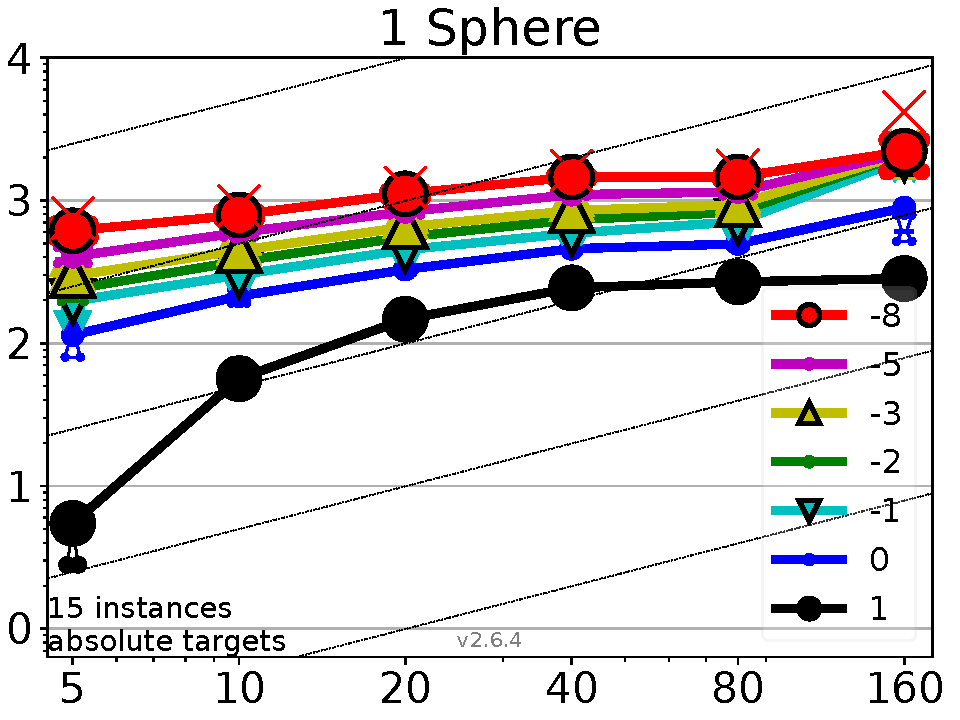
\includegraphics[width=0.19\textwidth]{ppfigdim_f001}&
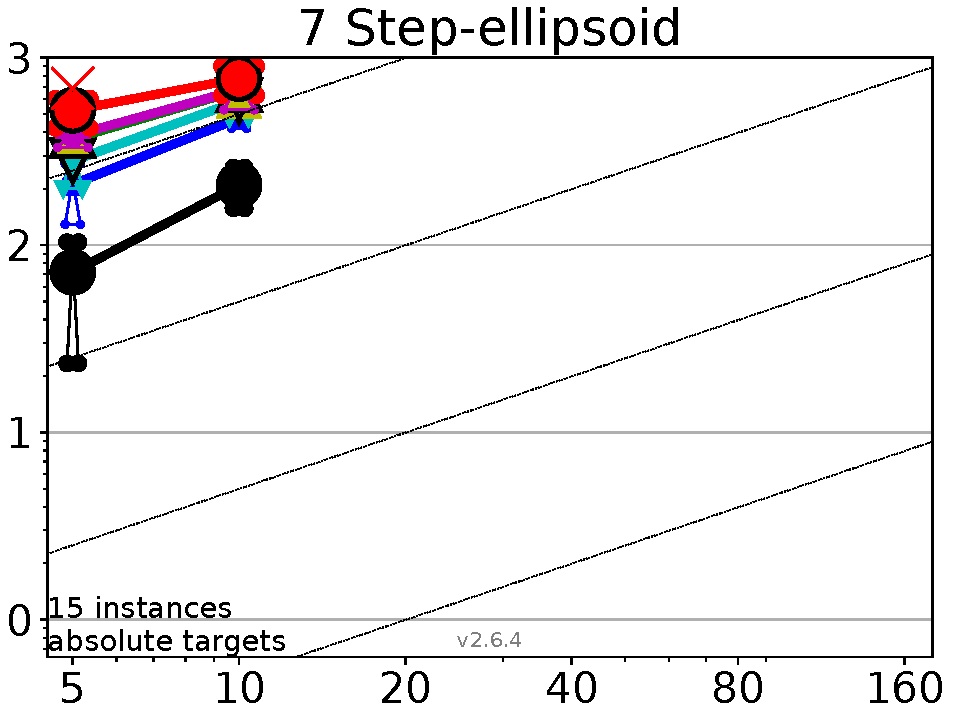
\includegraphics[width=0.19\textwidth]{ppfigdim_f007}&
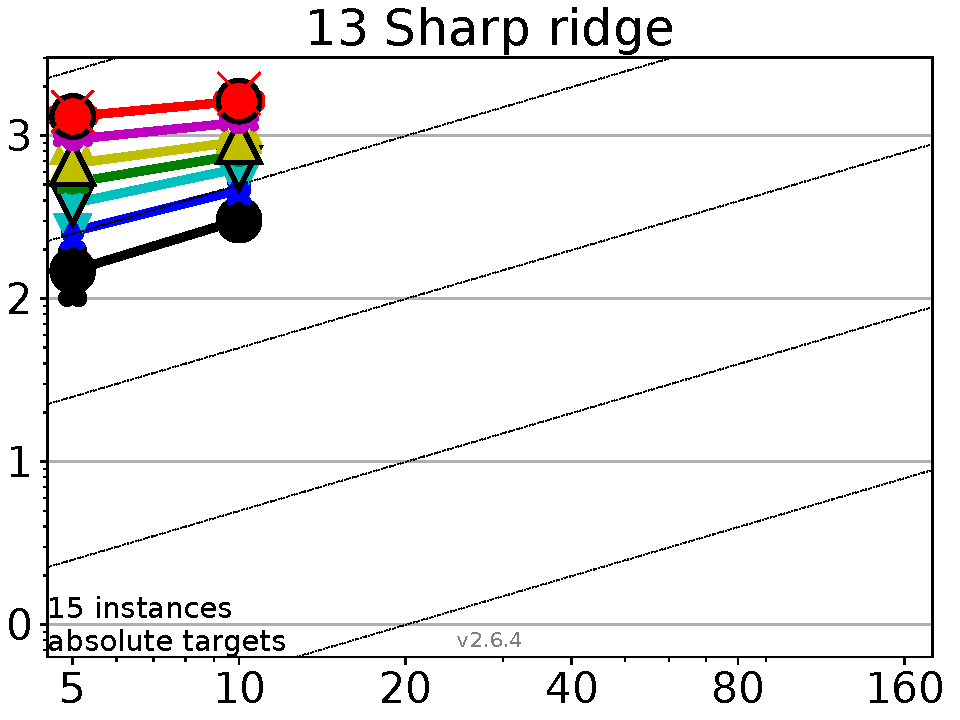
\includegraphics[width=0.19\textwidth]{ppfigdim_f013}&
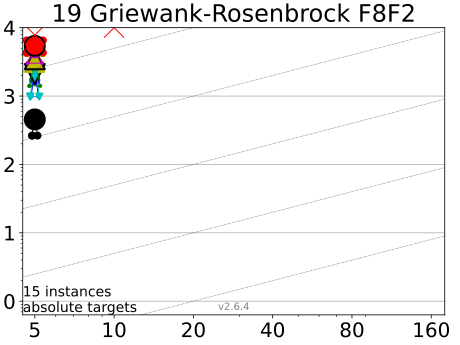
\includegraphics[width=0.19\textwidth]{ppfigdim_f019}&
\includegraphics[width=0.19\textwidth]{ppfigdim_f025}\\[-1ex]
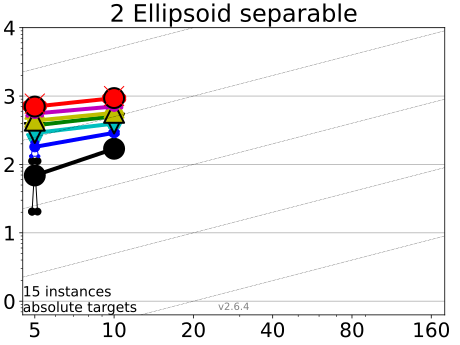
\includegraphics[width=0.19\textwidth]{ppfigdim_f002}&
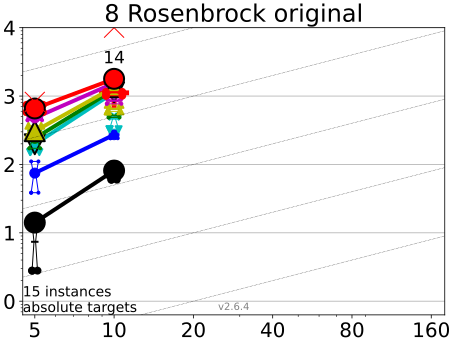
\includegraphics[width=0.19\textwidth]{ppfigdim_f008}&
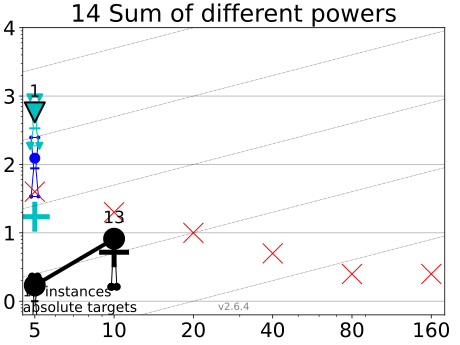
\includegraphics[width=0.19\textwidth]{ppfigdim_f014}&
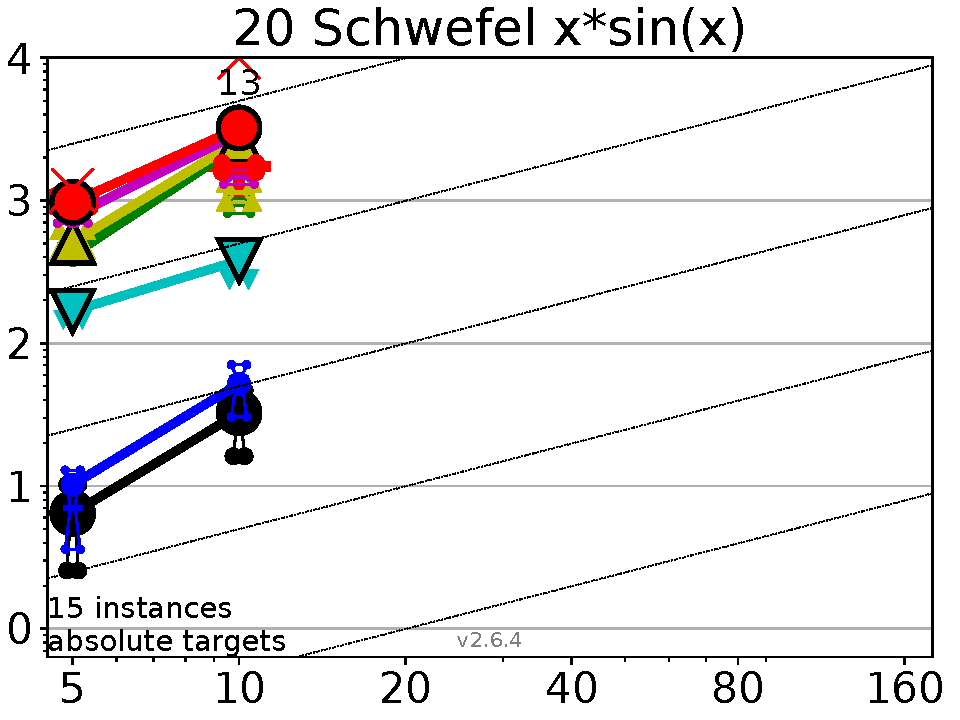
\includegraphics[width=0.19\textwidth]{ppfigdim_f020}&
\includegraphics[width=0.19\textwidth]{ppfigdim_f026}\\[-1ex]
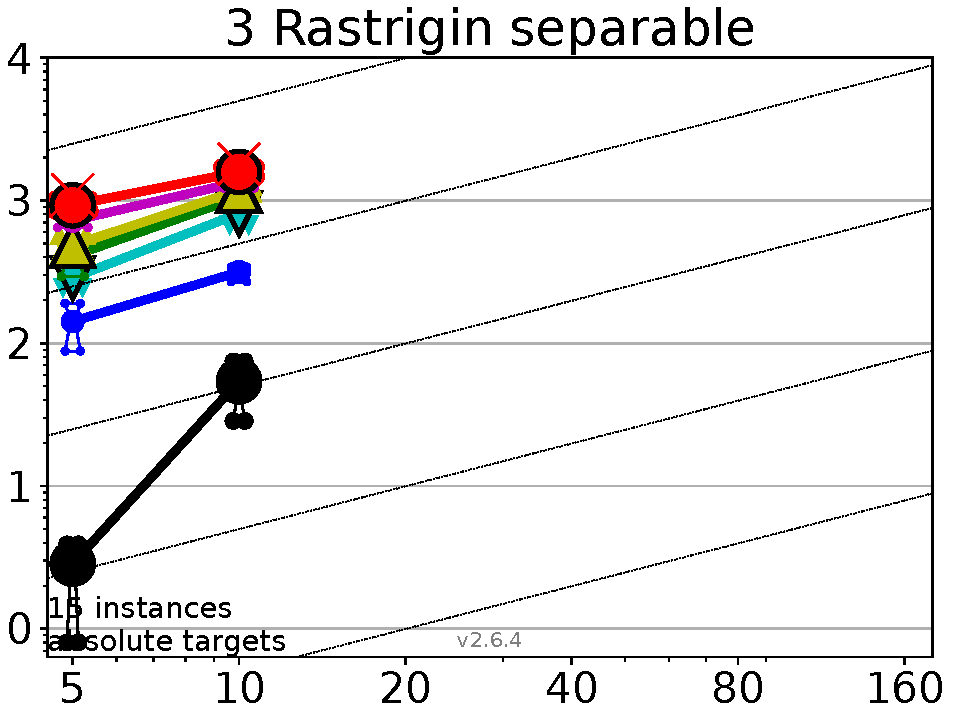
\includegraphics[width=0.19\textwidth]{ppfigdim_f003}&
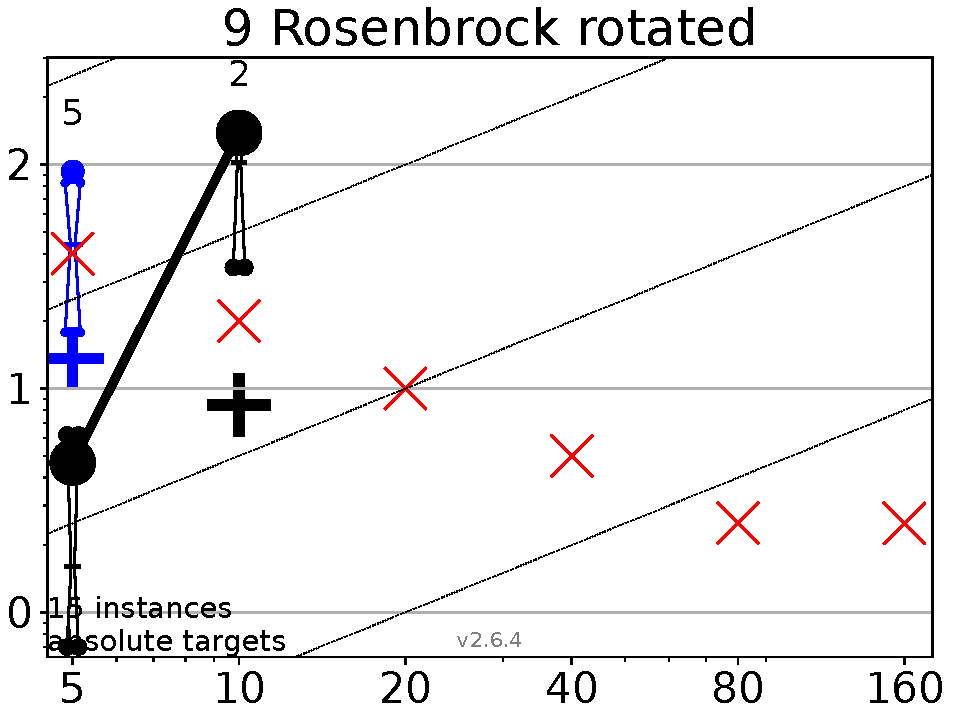
\includegraphics[width=0.19\textwidth]{ppfigdim_f009}&
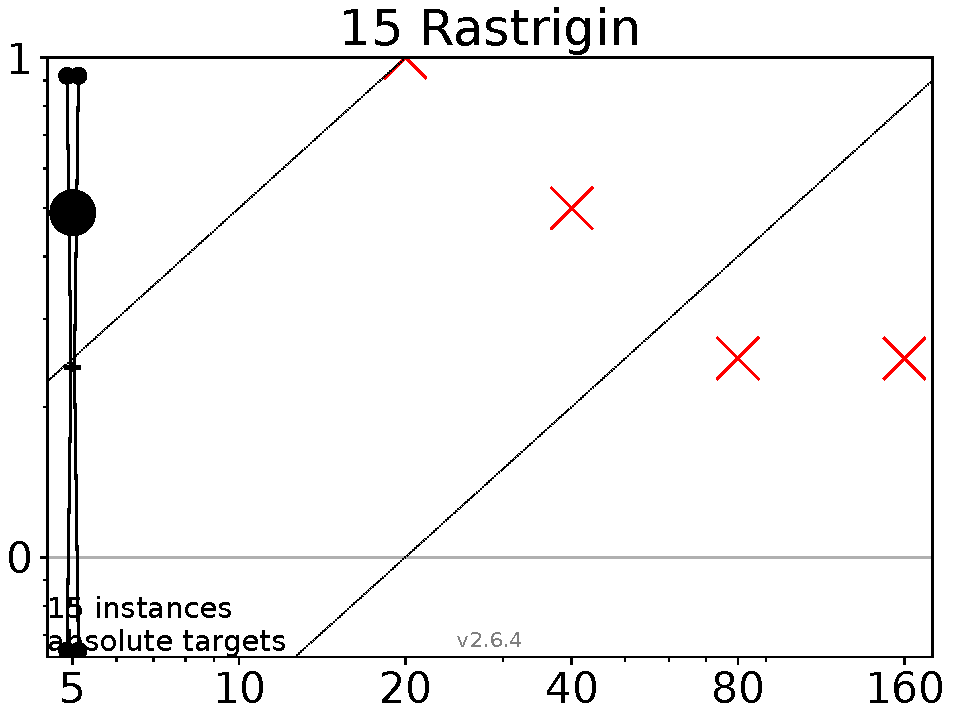
\includegraphics[width=0.19\textwidth]{ppfigdim_f015}&
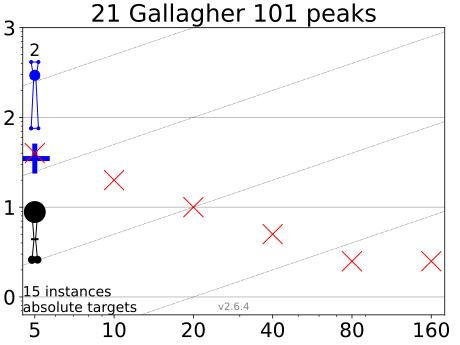
\includegraphics[width=0.19\textwidth]{ppfigdim_f021}&
\includegraphics[width=0.19\textwidth]{ppfigdim_f027}\\[-1ex]
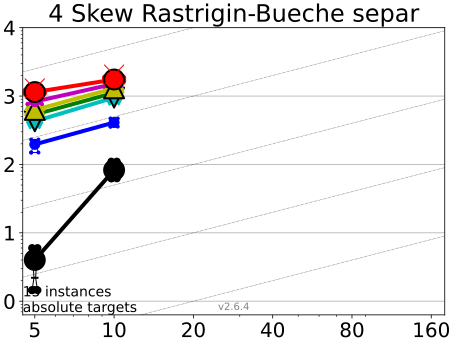
\includegraphics[width=0.19\textwidth]{ppfigdim_f004}&
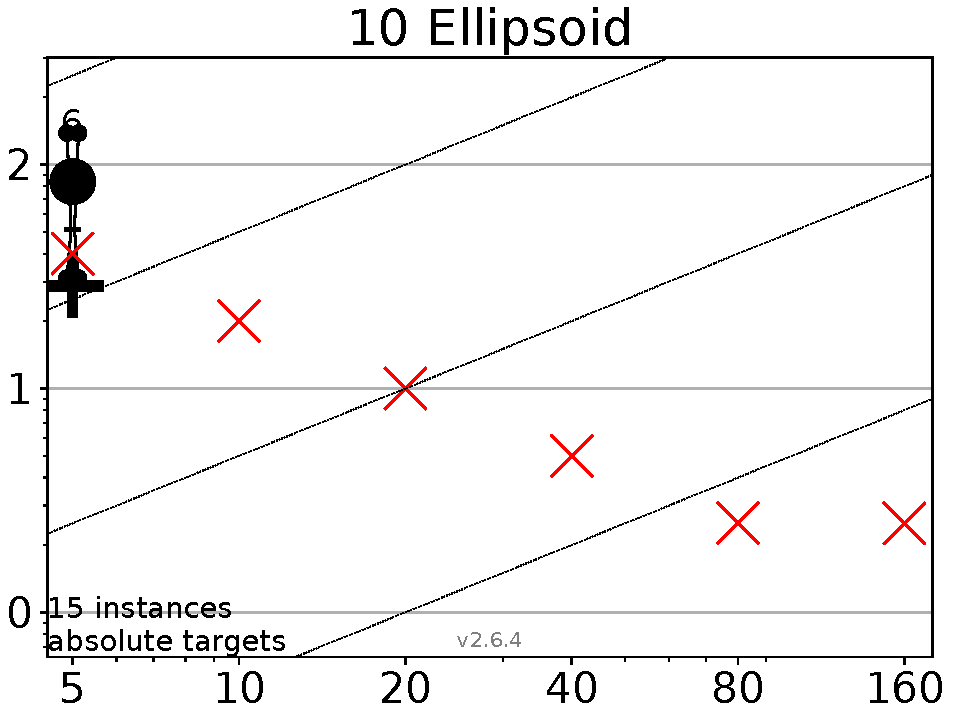
\includegraphics[width=0.19\textwidth]{ppfigdim_f010}&
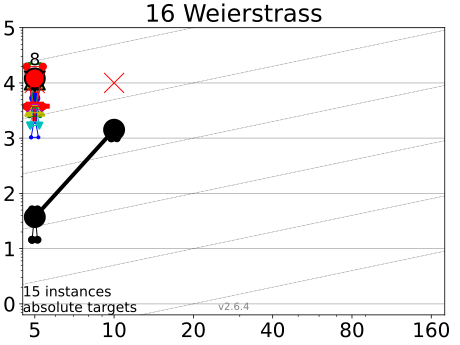
\includegraphics[width=0.19\textwidth]{ppfigdim_f016}&
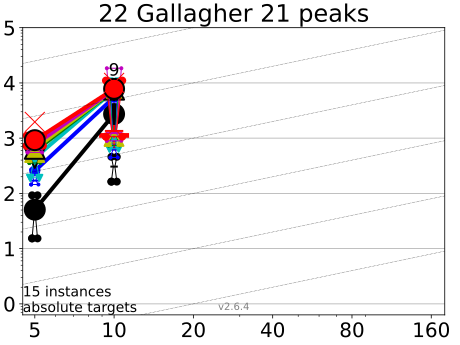
\includegraphics[width=0.19\textwidth]{ppfigdim_f022}&
\includegraphics[width=0.19\textwidth]{ppfigdim_f028}\\[-1ex]
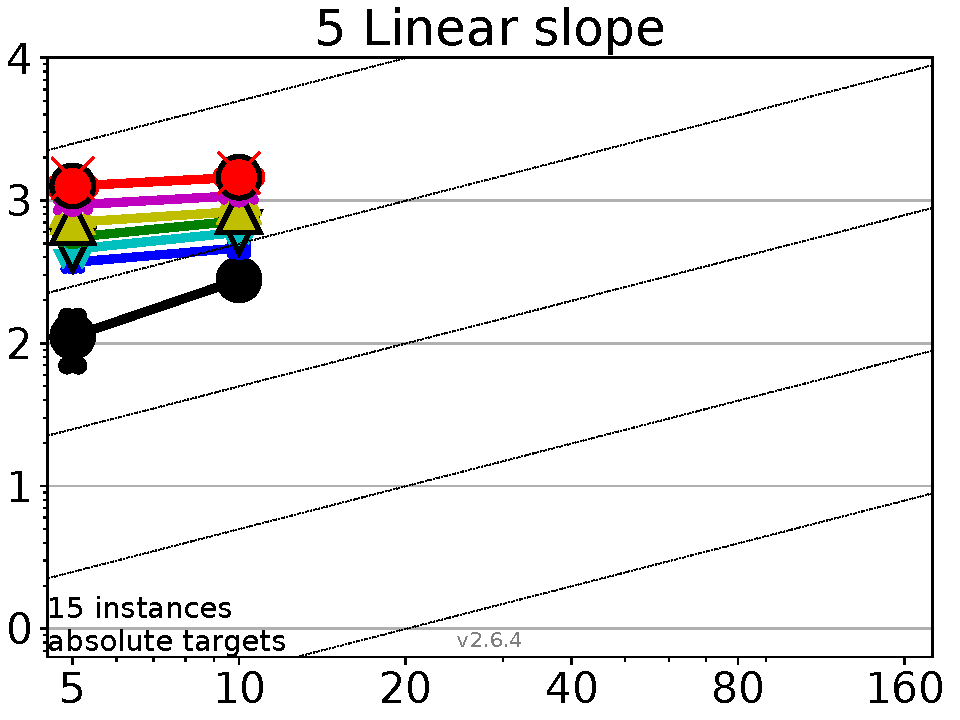
\includegraphics[width=0.19\textwidth]{ppfigdim_f005}&
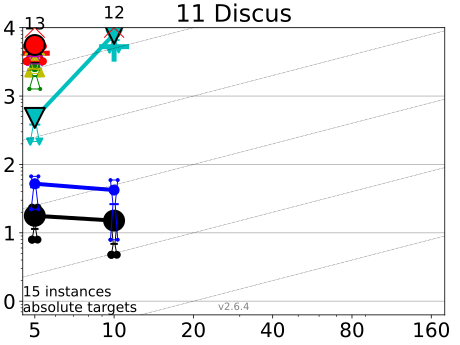
\includegraphics[width=0.19\textwidth]{ppfigdim_f011}&
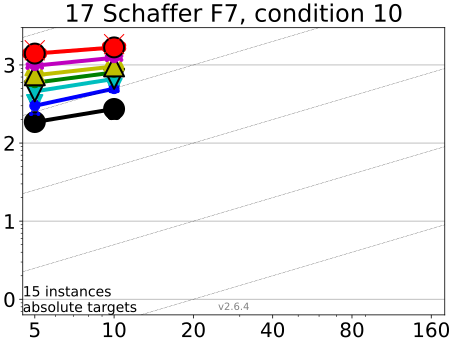
\includegraphics[width=0.19\textwidth]{ppfigdim_f017}&
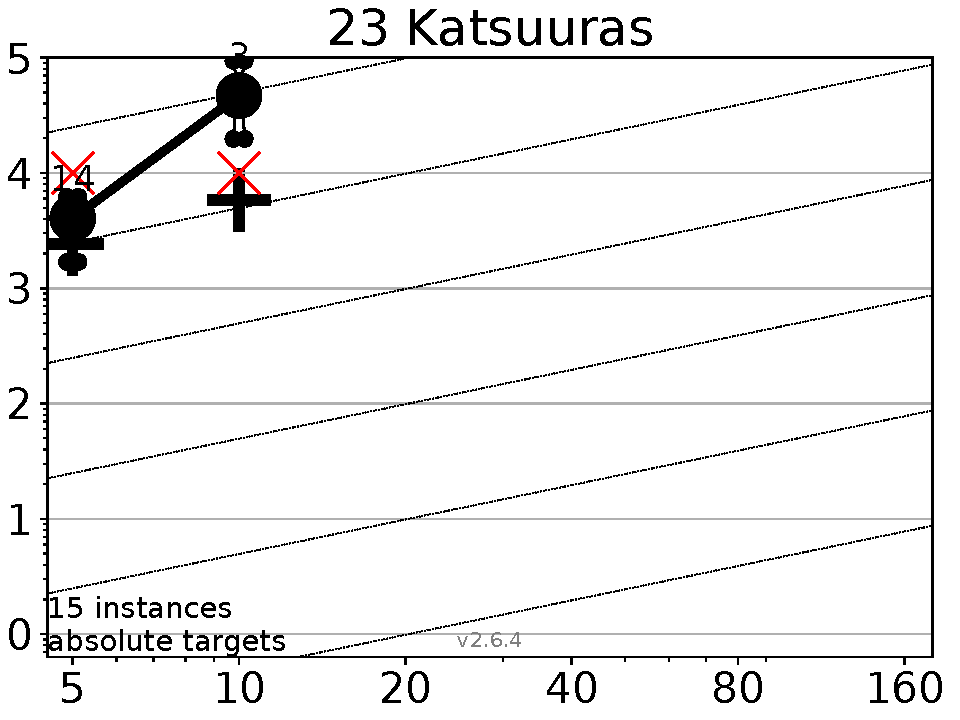
\includegraphics[width=0.19\textwidth]{ppfigdim_f023}&
\includegraphics[width=0.19\textwidth]{ppfigdim_f029}\\[-1ex]
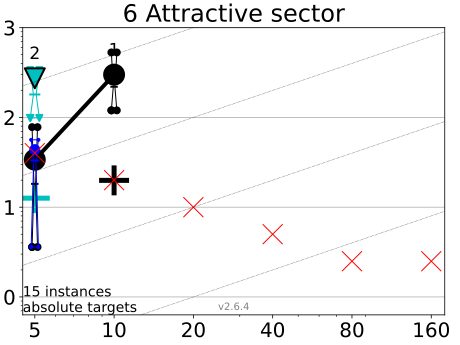
\includegraphics[width=0.19\textwidth]{ppfigdim_f006}&
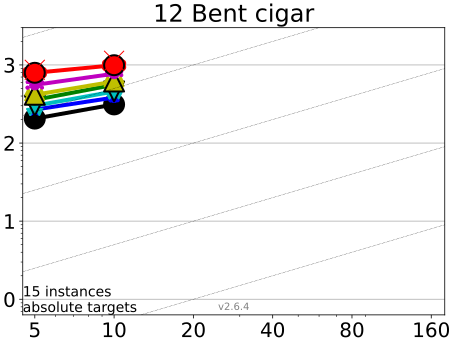
\includegraphics[width=0.19\textwidth]{ppfigdim_f012}&
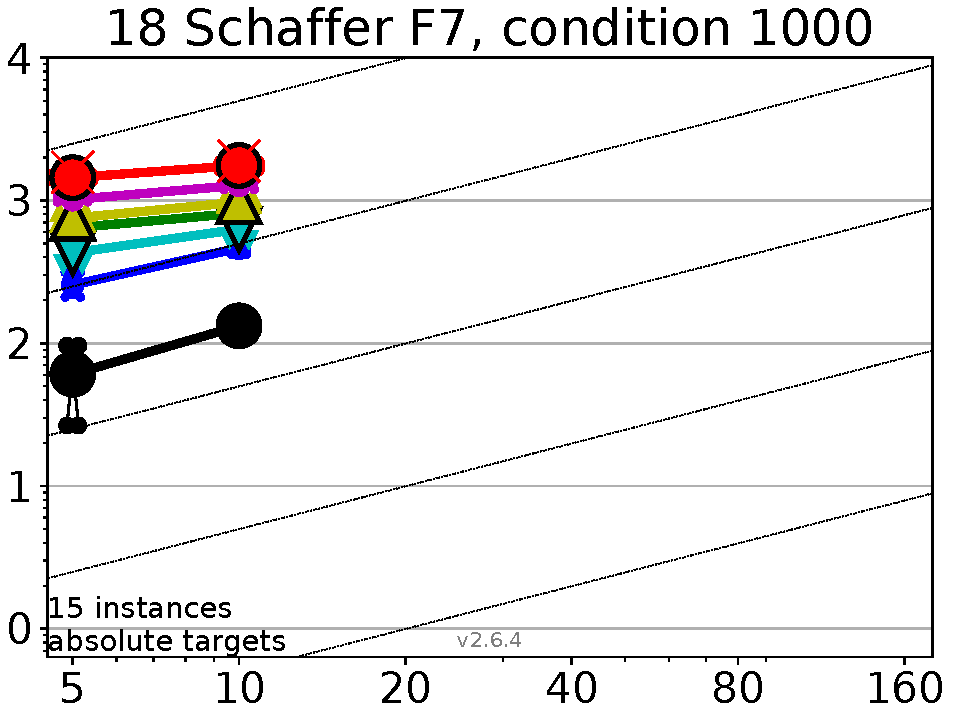
\includegraphics[width=0.19\textwidth]{ppfigdim_f018}&
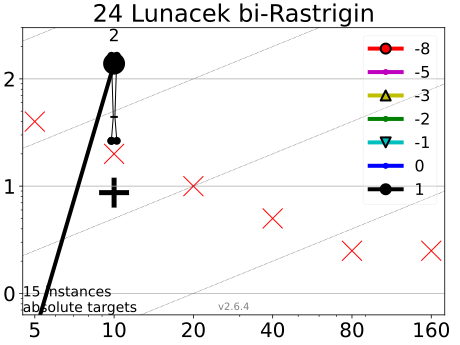
\includegraphics[width=0.19\textwidth]{ppfigdim_f024}&
\includegraphics[width=0.19\textwidth]{ppfigdim_f030}
\end{tabular}
\vspace{-3ex}
 \caption{\label{fig:ERTgraphsOne}
 \bbobppfigdimlegend{$f_1$}
 }
\end{figure*}

\begin{figure*}
\begin{tabular}{l@{\hspace*{-0.0\textwidth}}l@{\hspace*{-0.0\textwidth}}l@{\hspace*{-0.0\textwidth}}l}
\includegraphics[width=0.19\textwidth]{ppfigdim_f031}&
\includegraphics[width=0.19\textwidth]{ppfigdim_f037}&
\includegraphics[width=0.19\textwidth]{ppfigdim_f043}&
\includegraphics[width=0.19\textwidth]{ppfigdim_f049}\\[-1ex]
\includegraphics[width=0.19\textwidth]{ppfigdim_f032}&
\includegraphics[width=0.19\textwidth]{ppfigdim_f038}&
\includegraphics[width=0.19\textwidth]{ppfigdim_f044}&
\includegraphics[width=0.19\textwidth]{ppfigdim_f050}\\[-1ex]
\includegraphics[width=0.19\textwidth]{ppfigdim_f033}&
\includegraphics[width=0.19\textwidth]{ppfigdim_f039}&
\includegraphics[width=0.19\textwidth]{ppfigdim_f045}&
\includegraphics[width=0.19\textwidth]{ppfigdim_f051}\\[-1ex]
\includegraphics[width=0.19\textwidth]{ppfigdim_f034}&
\includegraphics[width=0.19\textwidth]{ppfigdim_f040}&
\includegraphics[width=0.19\textwidth]{ppfigdim_f046}&
\includegraphics[width=0.19\textwidth]{ppfigdim_f052}\\[-1ex]
\includegraphics[width=0.19\textwidth]{ppfigdim_f035}&
\includegraphics[width=0.19\textwidth]{ppfigdim_f041}&
\includegraphics[width=0.19\textwidth]{ppfigdim_f047}&
\includegraphics[width=0.19\textwidth]{ppfigdim_f053}\\[-1ex]
\includegraphics[width=0.19\textwidth]{ppfigdim_f036}&
\includegraphics[width=0.19\textwidth]{ppfigdim_f042}&
\includegraphics[width=0.19\textwidth]{ppfigdim_f048}&
\includegraphics[width=0.19\textwidth]{ppfigdim_f054}
\end{tabular}
\vspace{-3ex}
 \caption{\label{fig:ERTgraphsTwo}
 \bbobppfigdimlegend{$f_{54}$}
 }
\end{figure*}
%%%%%%%%%%%%%%%%%%%%%%%%%%%%%%%%%%%%%%%%%%%%%%%%%%%%%%%%%%%%%%%%%%%%%%%%%%%%%%%

%%%%%%%%%%%%%%%%%%%%%%%%%%%%%%%%%%%%%%%%%%%%%%%%%%%%%%%%%%%%%%%%%%%%%%%%%%%%%%%

% Scaling graphs with respect to the number of constraints
% in dimension 20

%%%%%%%%%%%%%%%%%%%%%%%%%%%%%%%%%%%%%%%%%%%%%%%%%%%%%%%%%%%%%%%%%%%%%%%%%%%%%%%

\begin{figure*}
 \begin{tabular}{@{}c@{}c@{}c@{}}
 \includegraphics[width=0.3\textwidth]{ppfigcons1_Sphere_d20} &
 \includegraphics[width=0.3\textwidth]{"ppfigcons1_Separable Ellipsoid_d20"} &
 \includegraphics[width=0.3\textwidth]{"ppfigcons1_Linear Slope_d20"}\\
 \includegraphics[width=0.3\textwidth]{"ppfigcons1_Rotated Ellipsoid_d20"} &
 \includegraphics[width=0.3\textwidth]{ppfigcons1_Discus_d20} &
 \includegraphics[width=0.3\textwidth]{"ppfigcons1_Bent Cigar_d20"}\\
 \includegraphics[width=0.3\textwidth]{"ppfigcons1_Different Powers_d20"} &
 \includegraphics[width=0.3\textwidth]{"ppfigcons1_Separable Rastrigin_d20"} &
 \includegraphics[width=0.3\textwidth]{"ppfigcons1_Rotated Rastrigin_d20"}\\
 \end{tabular}
\caption{
\label{fig:scalingconstraints20D}
Scaling of ERT divided by dimension with the number of constraints for all nine raw functions in the \bbobcons suite in dimension 20, for multiple targets, as in Figures~\ref{fig:ERTgraphsOne} and~\ref{fig:ERTgraphsTwo}. The vertical dashed lines depict the number of active (blue) and overall number (green) of constraints.
}
\end{figure*}
%%%%%%%%%%%%%%%%%%%%%%%%%%%%%%%%%%%%%%%%%%%%%%%%%%%%%%%%%%%%%%%%%%%%%%%%%%%%%%%

%%%%%%%%%%%%%%%%%%%%%%%%%%%%%%%%%%%%%%%%%%%%%%%%%%%%%%%%%%%%%%%%%%%%%%%%%%%%%%%

% ECDFs per function

%%%%%%%%%%%%%%%%%%%%%%%%%%%%%%%%%%%%%%%%%%%%%%%%%%%%%%%%%%%%%%%%%%%%%%%%%%%%%%%
\begin{figure*}
\centering
\begin{tabular}{l@{\hspace*{-0.00\textwidth}}l@{\hspace*{0.01\textwidth}}l@{\hspace*{-0.00\textwidth}}l@{\hspace*{-0.00\textwidth}}l}
\includegraphics[width=0.19\textwidth]{pprldmany-single-functions/pprldmany_f001}&
\includegraphics[width=0.19\textwidth]{pprldmany-single-functions/pprldmany_f007}&
\includegraphics[width=0.19\textwidth]{pprldmany-single-functions/pprldmany_f013}&
\includegraphics[width=0.19\textwidth]{pprldmany-single-functions/pprldmany_f019}&
\includegraphics[width=0.19\textwidth]{pprldmany-single-functions/pprldmany_f025}\\[-0.2em]
\includegraphics[width=0.19\textwidth]{pprldmany-single-functions/pprldmany_f002}&
\includegraphics[width=0.19\textwidth]{pprldmany-single-functions/pprldmany_f008}&
\includegraphics[width=0.19\textwidth]{pprldmany-single-functions/pprldmany_f014}&
\includegraphics[width=0.19\textwidth]{pprldmany-single-functions/pprldmany_f020}&
\includegraphics[width=0.19\textwidth]{pprldmany-single-functions/pprldmany_f026}\\[-0.2em]
\includegraphics[width=0.19\textwidth]{pprldmany-single-functions/pprldmany_f003}&
\includegraphics[width=0.19\textwidth]{pprldmany-single-functions/pprldmany_f009}&
\includegraphics[width=0.19\textwidth]{pprldmany-single-functions/pprldmany_f015}&
\includegraphics[width=0.19\textwidth]{pprldmany-single-functions/pprldmany_f021}&
\includegraphics[width=0.19\textwidth]{pprldmany-single-functions/pprldmany_f027}\\[-0.2em]
\includegraphics[width=0.19\textwidth]{pprldmany-single-functions/pprldmany_f004}&
\includegraphics[width=0.19\textwidth]{pprldmany-single-functions/pprldmany_f010}&
\includegraphics[width=0.19\textwidth]{pprldmany-single-functions/pprldmany_f016}&
\includegraphics[width=0.19\textwidth]{pprldmany-single-functions/pprldmany_f022}&
\includegraphics[width=0.19\textwidth]{pprldmany-single-functions/pprldmany_f028}\\[-0.2em]
\includegraphics[width=0.19\textwidth]{pprldmany-single-functions/pprldmany_f005}&
\includegraphics[width=0.19\textwidth]{pprldmany-single-functions/pprldmany_f011}&
\includegraphics[width=0.19\textwidth]{pprldmany-single-functions/pprldmany_f017}&
\includegraphics[width=0.19\textwidth]{pprldmany-single-functions/pprldmany_f023}&
\includegraphics[width=0.19\textwidth]{pprldmany-single-functions/pprldmany_f029}\\[-0.2em]
\includegraphics[width=0.19\textwidth]{pprldmany-single-functions/pprldmany_f006}&
\includegraphics[width=0.19\textwidth]{pprldmany-single-functions/pprldmany_f012}&
\includegraphics[width=0.19\textwidth]{pprldmany-single-functions/pprldmany_f018}&
\includegraphics[width=0.19\textwidth]{pprldmany-single-functions/pprldmany_f024}&
\includegraphics[width=0.19\textwidth]{pprldmany-single-functions/pprldmany_f030}
\vspace*{-1ex}
\end{tabular}
 \caption{\label{fig:ECDFsingleOne}
	\bbobecdfcaptionsinglefunctionssingledim{$\!\!$s 2 to 40 and problem IDs 1 to 30}
}
\end{figure*}

%%%%%%%%%%%%%%%%%%%%%%%%%%%%%%%%%%%%%%%%%%%%%%%%%%%%%%%%%%%%%%%%%%%%%%%%%%%%%%%
\begin{figure*}
\centering
\begin{tabular}{l@{\hspace*{-0.00\textwidth}}l@{\hspace*{0.01\textwidth}}l@{\hspace*{-0.00\textwidth}}l}
\includegraphics[width=0.19\textwidth]{pprldmany-single-functions/pprldmany_f031}&
\includegraphics[width=0.19\textwidth]{pprldmany-single-functions/pprldmany_f037}&
\includegraphics[width=0.19\textwidth]{pprldmany-single-functions/pprldmany_f043}&
\includegraphics[width=0.19\textwidth]{pprldmany-single-functions/pprldmany_f049}\\[-0.2em]
\includegraphics[width=0.19\textwidth]{pprldmany-single-functions/pprldmany_f032}&
\includegraphics[width=0.19\textwidth]{pprldmany-single-functions/pprldmany_f038}&
\includegraphics[width=0.19\textwidth]{pprldmany-single-functions/pprldmany_f044}&
\includegraphics[width=0.19\textwidth]{pprldmany-single-functions/pprldmany_f050}\\[-0.2em]
\includegraphics[width=0.19\textwidth]{pprldmany-single-functions/pprldmany_f033}&
\includegraphics[width=0.19\textwidth]{pprldmany-single-functions/pprldmany_f039}&
\includegraphics[width=0.19\textwidth]{pprldmany-single-functions/pprldmany_f045}&
\includegraphics[width=0.19\textwidth]{pprldmany-single-functions/pprldmany_f051}\\[-0.2em]
\includegraphics[width=0.19\textwidth]{pprldmany-single-functions/pprldmany_f034}&
\includegraphics[width=0.19\textwidth]{pprldmany-single-functions/pprldmany_f040}&
\includegraphics[width=0.19\textwidth]{pprldmany-single-functions/pprldmany_f046}&
\includegraphics[width=0.19\textwidth]{pprldmany-single-functions/pprldmany_f052}\\[-0.2em]
\includegraphics[width=0.19\textwidth]{pprldmany-single-functions/pprldmany_f035}&
\includegraphics[width=0.19\textwidth]{pprldmany-single-functions/pprldmany_f042}&
\includegraphics[width=0.19\textwidth]{pprldmany-single-functions/pprldmany_f048}&
\includegraphics[width=0.19\textwidth]{pprldmany-single-functions/pprldmany_f052}\\[-0.2em]
\includegraphics[width=0.19\textwidth]{pprldmany-single-functions/pprldmany_f036}&
\includegraphics[width=0.19\textwidth]{pprldmany-single-functions/pprldmany_f042}&
\includegraphics[width=0.19\textwidth]{pprldmany-single-functions/pprldmany_f048}&
\includegraphics[width=0.19\textwidth]{pprldmany-single-functions/pprldmany_f054}
\vspace*{-1ex}
\end{tabular}
 \caption{\label{fig:ECDFsingleTwo}
   \bbobecdfcaptionsinglefunctionssingledim{$\!\!$s 2 to 40 and problem IDs 31 to 54}
}
\end{figure*}
%%%%%%%%%%%%%%%%%%%%%%%%%%%%%%%%%%%%%%%%%%%%%%%%%%%%%%%%%%%%%%%%%%%%%%%%%%%%%%%
}{} % end of 1 algorithm template





\ifthenelse{\numofalgs > 1}{

%%%%%%%%%%%%%%%%%%%%%%%%%%%%%%%%%%%%%%%%%%%%%%%%%%%%%%%%%%%%%%%%%%%%%%%%%%%%%%%
%%%%%%%%%%%%%%%%%%%%%%%%%%%%%%%%%%%%%%%%%%%%%%%%%%%%%%%%%%%%%%%%%%%%%%%%%%%%%%%

% Scaling of ERT with dimension

%%%%%%%%%%%%%%%%%%%%%%%%%%%%%%%%%%%%%%%%%%%%%%%%%%%%%%%%%%%%%%%%%%%%%%%%%%%%%%%

\begin{figure*}
\centering
\begin{tabular}{@{}c@{}c@{}c@{}c@{}c@{}}
\includegraphics[width=0.19\textwidth]{ppfigs_f001}&
\includegraphics[width=0.19\textwidth]{ppfigs_f007}&
\includegraphics[width=0.19\textwidth]{ppfigs_f013}&
\includegraphics[width=0.19\textwidth]{ppfigs_f019}&
\includegraphics[width=0.19\textwidth]{ppfigs_f025}\\[-0.25em]
\includegraphics[width=0.19\textwidth]{ppfigs_f002}&
\includegraphics[width=0.19\textwidth]{ppfigs_f008}&
\includegraphics[width=0.19\textwidth]{ppfigs_f014}&
\includegraphics[width=0.19\textwidth]{ppfigs_f020}&
\includegraphics[width=0.19\textwidth]{ppfigs_f026}\\[-0.25em]
\includegraphics[width=0.19\textwidth]{ppfigs_f003}&
\includegraphics[width=0.19\textwidth]{ppfigs_f009}&
\includegraphics[width=0.19\textwidth]{ppfigs_f015}&
\includegraphics[width=0.19\textwidth]{ppfigs_f021}&
\includegraphics[width=0.19\textwidth]{ppfigs_f027}\\[-0.25em]
\includegraphics[width=0.19\textwidth]{ppfigs_f004}&
\includegraphics[width=0.19\textwidth]{ppfigs_f010}&
\includegraphics[width=0.19\textwidth]{ppfigs_f016}&
\includegraphics[width=0.19\textwidth]{ppfigs_f022}&
\includegraphics[width=0.19\textwidth]{ppfigs_f018}\\[-0.25em]
\includegraphics[width=0.19\textwidth]{ppfigs_f005}&
\includegraphics[width=0.19\textwidth]{ppfigs_f011}&
\includegraphics[width=0.19\textwidth]{ppfigs_f017}&
\includegraphics[width=0.19\textwidth]{ppfigs_f023}&
\includegraphics[width=0.19\textwidth]{ppfigs_f029}\\[-0.25em]
\includegraphics[width=0.19\textwidth]{ppfigs_f006}&
\includegraphics[width=0.19\textwidth]{ppfigs_f012}&
\includegraphics[width=0.19\textwidth]{ppfigs_f018}&
\includegraphics[width=0.19\textwidth]{ppfigs_f024}&
\includegraphics[width=0.19\textwidth]{ppfigs_f030}
\end{tabular}
\vspace*{-0.2cm}
\caption[Expected running time (\ERT) divided by dimension
versus dimension in log-log presentation]{
\label{fig:scaling}
\bbobppfigslegend{$f_1$}. 
}
% 
\end{figure*}


%%%%%%%%%%%%%%%%%%%%%%%%%%%%%%%%%%%%%%%%%%%%%%%%%%%%%%%%%%%%%%%%%%%%%%%%%%%%%%%
%%%%%%%%%%%%%%%%%%%%%%%%%%%%%%%%%%%%%%%%%%%%%%%%%%%%%%%%%%%%%%%%%%%%%%%%%%%%%%%

% Scaling of ERT with dimension, 2nd half

%%%%%%%%%%%%%%%%%%%%%%%%%%%%%%%%%%%%%%%%%%%%%%%%%%%%%%%%%%%%%%%%%%%%%%%%%%%%%%%

\begin{figure*}
\centering
\begin{tabular}{@{}c@{}c@{}c@{}c@{}c@{}}
\includegraphics[width=0.19\textwidth]{ppfigs_f031}&
\includegraphics[width=0.19\textwidth]{ppfigs_f037}&
\includegraphics[width=0.19\textwidth]{ppfigs_f043}&
\includegraphics[width=0.19\textwidth]{ppfigs_f049}\\[-0.25em]
\includegraphics[width=0.19\textwidth]{ppfigs_f032}&
\includegraphics[width=0.19\textwidth]{ppfigs_f038}&
\includegraphics[width=0.19\textwidth]{ppfigs_f044}&
\includegraphics[width=0.19\textwidth]{ppfigs_f050}\\[-0.25em]
\includegraphics[width=0.19\textwidth]{ppfigs_f033}&
\includegraphics[width=0.19\textwidth]{ppfigs_f039}&
\includegraphics[width=0.19\textwidth]{ppfigs_f045}&
\includegraphics[width=0.19\textwidth]{ppfigs_f051}\\[-0.25em]
\includegraphics[width=0.19\textwidth]{ppfigs_f034}&
\includegraphics[width=0.19\textwidth]{ppfigs_f040}&
\includegraphics[width=0.19\textwidth]{ppfigs_f046}&
\includegraphics[width=0.19\textwidth]{ppfigs_f052}\\[-0.25em]
\includegraphics[width=0.19\textwidth]{ppfigs_f035}&
\includegraphics[width=0.19\textwidth]{ppfigs_f041}&
\includegraphics[width=0.19\textwidth]{ppfigs_f047}&
\includegraphics[width=0.19\textwidth]{ppfigs_f053}\\[-0.25em]
\includegraphics[width=0.19\textwidth]{ppfigs_f036}&
\includegraphics[width=0.19\textwidth]{ppfigs_f042}&
\includegraphics[width=0.19\textwidth]{ppfigs_f048}&
\includegraphics[width=0.19\textwidth]{ppfigs_f054}
\end{tabular}
\vspace*{-0.2cm}
\caption[Expected running time (\ERT) divided by dimension
versus dimension in log-log presentation]{
\label{fig:scaling2}
\bbobppfigslegend{$f_{54}$}. 
}
% 
\end{figure*}
%%%%%%%%%%%%%%%%%%%%%%%%%%%%%%%%%%%%%%%%%%%%%%%%%%%%%%%%%%%%%%%%%%%%%%%%%%%%%%%

%%%%%%%%%%%%%%%%%%%%%%%%%%%%%%%%%%%%%%%%%%%%%%%%%%%%%%%%%%%%%%%%%%%%%%%%%%%%%%%
 
% Scaling graphs with respect to the number of constraints
% in dimension 20

%%%%%%%%%%%%%%%%%%%%%%%%%%%%%%%%%%%%%%%%%%%%%%%%%%%%%%%%%%%%%%%%%%%%%%%%%%%%%%%

\begin{figure*}
 \begin{tabular}{@{}c@{}c@{}c@{}}
 \includegraphics[width=0.3\textwidth]{ppfigcons_Sphere_d20} & 
 \includegraphics[width=0.3\textwidth]{"ppfigcons_Separable Ellipsoid_d20"} &
 \includegraphics[width=0.3\textwidth]{"ppfigcons_Linear Slope_d20"}\\
 \includegraphics[width=0.3\textwidth]{"ppfigcons_Rotated Ellipsoid_d20"} & 
 \includegraphics[width=0.3\textwidth]{ppfigcons_Discus_d20} &
 \includegraphics[width=0.3\textwidth]{"ppfigcons_Bent Cigar_d20"}\\ 
 \includegraphics[width=0.3\textwidth]{"ppfigcons_Different Powers_d20"} & 
 \includegraphics[width=0.3\textwidth]{"ppfigcons_Separable Rastrigin_d20"} &
 \includegraphics[width=0.3\textwidth]{"ppfigcons_Rotated Rastrigin_d20"}\\ 
 \end{tabular}
\caption{
\label{fig:scalingconstraints20D}
Scaling of ERT divided by dimension with the number of constraints for all nine raw functions in the \bbobcons suite, in dimension 20 for a single target. The vertical dashed lines depict the number of active (blue) and overall number (green) of constraints.
}
\end{figure*}
%%%%%%%%%%%%%%%%%%%%%%%%%%%%%%%%%%%%%%%%%%%%%%%%%%%%%%%%%%%%%%%%%%%%%%%%%%%%%%%

%%%%%%%%%%%%%%%%%%%%%%%%%%%%%%%%%%%%%%%%%%%%%%%%%%%%%%%%%%%%%%%%%%%%%%%%%%%%%%%

% ECDFs per function in dimension 20, part I

%%%%%%%%%%%%%%%%%%%%%%%%%%%%%%%%%%%%%%%%%%%%%%%%%%%%%%%%%%%%%%%%%%%%%%%%%%%%%%%
\begin{figure*}
\centering
\begin{tabular}{@{}l@{}l@{}l@{}l@{}l@{}}
\includegraphics[height=0.135\textwidth]{pprldmany-single-functions/pprldmany_f001_20D}&
\includegraphics[height=0.135\textwidth]{pprldmany-single-functions/pprldmany_f007_20D}&
\includegraphics[height=0.135\textwidth]{pprldmany-single-functions/pprldmany_f013_20D}&
\includegraphics[height=0.135\textwidth]{pprldmany-single-functions/pprldmany_f019_20D}&
\includegraphics[height=0.135\textwidth]{pprldmany-single-functions/pprldmany_f025_20D}\\
\includegraphics[height=0.135\textwidth]{pprldmany-single-functions/pprldmany_f002_20D}&
\includegraphics[height=0.135\textwidth]{pprldmany-single-functions/pprldmany_f008_20D}&
\includegraphics[height=0.135\textwidth]{pprldmany-single-functions/pprldmany_f014_20D}&
\includegraphics[height=0.135\textwidth]{pprldmany-single-functions/pprldmany_f020_20D}&
\includegraphics[height=0.135\textwidth]{pprldmany-single-functions/pprldmany_f026_20D}\\
\includegraphics[height=0.135\textwidth]{pprldmany-single-functions/pprldmany_f003_20D}&
\includegraphics[height=0.135\textwidth]{pprldmany-single-functions/pprldmany_f009_20D}&
\includegraphics[height=0.135\textwidth]{pprldmany-single-functions/pprldmany_f015_20D}&
\includegraphics[height=0.135\textwidth]{pprldmany-single-functions/pprldmany_f021_20D}&
\includegraphics[height=0.135\textwidth]{pprldmany-single-functions/pprldmany_f027_20D}\\
\blueline
\includegraphics[height=0.135\textwidth]{pprldmany-single-functions/pprldmany_f004_20D}&
\includegraphics[height=0.135\textwidth]{pprldmany-single-functions/pprldmany_f010_20D}&
\includegraphics[height=0.135\textwidth]{pprldmany-single-functions/pprldmany_f016_20D}&
\includegraphics[height=0.135\textwidth]{pprldmany-single-functions/pprldmany_f022_20D}&
\includegraphics[height=0.135\textwidth]{pprldmany-single-functions/pprldmany_f028_20D}\\
\greenline
\includegraphics[height=0.135\textwidth]{pprldmany-single-functions/pprldmany_f005_20D}&
\includegraphics[height=0.135\textwidth]{pprldmany-single-functions/pprldmany_f011_20D}&
\includegraphics[height=0.135\textwidth]{pprldmany-single-functions/pprldmany_f017_20D}&
\includegraphics[height=0.135\textwidth]{pprldmany-single-functions/pprldmany_f023_20D}&
\includegraphics[height=0.135\textwidth]{pprldmany-single-functions/pprldmany_f029_20D}\\
\includegraphics[height=0.135\textwidth]{pprldmany-single-functions/pprldmany_f006_20D}&
\includegraphics[height=0.135\textwidth]{pprldmany-single-functions/pprldmany_f012_20D}&
\includegraphics[height=0.135\textwidth]{pprldmany-single-functions/pprldmany_f018_20D}&
\includegraphics[height=0.135\textwidth]{pprldmany-single-functions/pprldmany_f024_20D}&
\includegraphics[height=0.135\textwidth]{pprldmany-single-functions/pprldmany_f030_20D}\\
\end{tabular}
 \caption{\label{fig:ECDFsingleOne}
	\bbobecdfcaptionsinglefunctionssingledim{20 and problem IDs 1 to 30}
   Above the blue (rsp. green) line are problems where there are less overall (rsp. active) constraints than dimension.
}
\end{figure*}

%%%%%%%%%%%%%%%%%%%%%%%%%%%%%%%%%%%%%%%%%%%%%%%%%%%%%%%%%%%%%%%%%%%%%%%%%%%%%%%
%%%%%%%%%%%%%%%%%%%%%%%%%%%%%%%%%%%%%%%%%%%%%%%%%%%%%%%%%%%%%%%%%%%%%%%%%%%%%%%

% ECDFs per function in dimension 20, part II

%%%%%%%%%%%%%%%%%%%%%%%%%%%%%%%%%%%%%%%%%%%%%%%%%%%%%%%%%%%%%%%%%%%%%%%%%%%%%%%
\begin{figure*}
\centering
\begin{tabular}{@{}l@{}l@{}l@{}l@{}l@{}}
\includegraphics[height=0.135\textwidth]{pprldmany-single-functions/pprldmany_f031_20D}&
\includegraphics[height=0.135\textwidth]{pprldmany-single-functions/pprldmany_f037_20D}&
\includegraphics[height=0.135\textwidth]{pprldmany-single-functions/pprldmany_f043_20D}&
\includegraphics[height=0.135\textwidth]{pprldmany-single-functions/pprldmany_f049_20D}\\
\includegraphics[height=0.135\textwidth]{pprldmany-single-functions/pprldmany_f032_20D}&
\includegraphics[height=0.135\textwidth]{pprldmany-single-functions/pprldmany_f038_20D}&
\includegraphics[height=0.135\textwidth]{pprldmany-single-functions/pprldmany_f044_20D}&
\includegraphics[height=0.135\textwidth]{pprldmany-single-functions/pprldmany_f050_20D}\\
\includegraphics[height=0.135\textwidth]{pprldmany-single-functions/pprldmany_f033_20D}&
\includegraphics[height=0.135\textwidth]{pprldmany-single-functions/pprldmany_f039_20D}&
\includegraphics[height=0.135\textwidth]{pprldmany-single-functions/pprldmany_f045_20D}&
\includegraphics[height=0.135\textwidth]{pprldmany-single-functions/pprldmany_f051_20D}\\
\blueline
\includegraphics[height=0.135\textwidth]{pprldmany-single-functions/pprldmany_f034_20D}&
\includegraphics[height=0.135\textwidth]{pprldmany-single-functions/pprldmany_f040_20D}&
\includegraphics[height=0.135\textwidth]{pprldmany-single-functions/pprldmany_f046_20D}&
\includegraphics[height=0.135\textwidth]{pprldmany-single-functions/pprldmany_f052_20D}\\
\greenline
\includegraphics[height=0.135\textwidth]{pprldmany-single-functions/pprldmany_f035_20D}&
\includegraphics[height=0.135\textwidth]{pprldmany-single-functions/pprldmany_f041_20D}&
\includegraphics[height=0.135\textwidth]{pprldmany-single-functions/pprldmany_f047_20D}&
\includegraphics[height=0.135\textwidth]{pprldmany-single-functions/pprldmany_f053_20D}\\
\includegraphics[height=0.135\textwidth]{pprldmany-single-functions/pprldmany_f036_20D}&
\includegraphics[height=0.135\textwidth]{pprldmany-single-functions/pprldmany_f042_20D}&
\includegraphics[height=0.135\textwidth]{pprldmany-single-functions/pprldmany_f048_20D}&
\includegraphics[height=0.135\textwidth]{pprldmany-single-functions/pprldmany_f054_20D}\\
\end{tabular}
 \caption{\label{fig:ECDFsingleTwo}
   \bbobecdfcaptionsinglefunctionssingledim{20 and problem IDs 31 to 54}
   Above the blue (rsp. green) line are problems where there are less overall (rsp. active) constraints than dimension.
}
\end{figure*}
%%%%%%%%%%%%%%%%%%%%%%%%%%%%%%%%%%%%%%%%%%%%%%%%%%%%%%%%%%%%%%%%%%%%%%%%%%%%%%%


}{} % end of all that comes for 2 or 3+ algorithms



\ifthenelse{\numofalgs = 2}{


%%%%%%%%%%%%%%%%%%%%%%%%%%%%%%%%%%%%%%%%%%%%%%%%%%%%%%%%%%%%%%%%%%%%%%%%%%%%%%%
%%%%%%%%%%%%%%%%%%%%%%%%%%%%%%%%%%%%%%%%%%%%%%%%%%%%%%%%%%%%%%%%%%%%%%%%%%%%%%%
 
% Scatter plots per function.

%%%%%%%%%%%%%%%%%%%%%%%%%%%%%%%%%%%%%%%%%%%%%%%%%%%%%%%%%%%%%%%%%%%%%%%%%%%%%%%

%%%%%%%%%%%%%%%%%%%%%%%%%%%%%%%%%%%%%%%%%%%%%%%%%%%%%%%%%%%%%%%%%%%%%%%%%%%%%%%
%%%%%%%%%%%%%%%%%%%%%%%%%%%%%%%%%%%%%%%%%%%%%%%%%%%%%%%%%%%%%%%%%%%%%%%%%%%%%%%
%%%%%%%%%%%%%%%%%%%%%%%%%%%%%%%%%%%%%%%%%%%%%%%%%%%%%%%%%%%%%%%%%%%%%%%%%%%%%%%

\begin{figure*}
\begin{tabular}{*{4}{@{}c@{}}}
    \includegraphics[height=0.2\textwidth]{ppscatter_f001}&
    \includegraphics[height=0.2\textwidth]{ppscatter_f002}&
    \includegraphics[height=0.2\textwidth]{ppscatter_f003}&
    \includegraphics[height=0.2\textwidth]{ppscatter_f004}\\[-0.6em]
    \includegraphics[height=0.2\textwidth]{ppscatter_f005}&
    \includegraphics[height=0.2\textwidth]{ppscatter_f006}&
    \includegraphics[height=0.2\textwidth]{ppscatter_f007}&
    \includegraphics[height=0.2\textwidth]{ppscatter_f008}\\[-0.6em]
    \includegraphics[height=0.2\textwidth]{ppscatter_f009}&
    \includegraphics[height=0.2\textwidth]{ppscatter_f010}&
    \includegraphics[height=0.2\textwidth]{ppscatter_f011}&
    \includegraphics[height=0.2\textwidth]{ppscatter_f012}\\[-0.6em]
    \includegraphics[height=0.2\textwidth]{ppscatter_f013}&
    \includegraphics[height=0.2\textwidth]{ppscatter_f014}&
    \includegraphics[height=0.2\textwidth]{ppscatter_f015}&
    \includegraphics[height=0.2\textwidth]{ppscatter_f016}\\[-0.6em]
    \includegraphics[height=0.2\textwidth]{ppscatter_f017}&
    \includegraphics[height=0.2\textwidth]{ppscatter_f018}&
    \includegraphics[height=0.2\textwidth]{ppscatter_f019}&
    \includegraphics[height=0.2\textwidth]{ppscatter_f020}\\[-0.6em]
    \includegraphics[height=0.2\textwidth]{ppscatter_f021}&
    \includegraphics[height=0.2\textwidth]{ppscatter_f022}&
    \includegraphics[height=0.2\textwidth]{ppscatter_f023}&
    \includegraphics[height=0.2\textwidth]{ppscatter_f024}
\end{tabular}
\caption{\label{fig:scatterplots}
\bbobppscatterlegend{$f_1$--$f_{24}$}
}
\end{figure*}



} % end of 2 algorithms template




%%%%%%%%%%%%%%%%%%%%%%%%%%%%%%%%%%%%%%%%%%%%%%%%%%%%%%%%%%%%%%%%%%%%%%%%%%%%%%%
%%%%%%%%%%%%%%%%%%%%%%%%%%%%%%%%%%%%%%%%%%%%%%%%%%%%%%%%%%%%%%%%%%%%%%%%%%%%%%%

\bibliographystyle{ACM-Reference-Format}
\bibliography{bbob}  % bbob.bib is the name of the Bibliography in this case

%%%%%%%%%%%%%%%%%%%%%%%%%%%%%%%%%%%%%%%%%%%%%%%%%%%%%%%%%%%%%%%%%%%%%%%%%%%%%%%%%%%%%%%%%%%


%%%%%%%%%%%%%%%%%%%%%%%%%%%%%%%%%%%%%%%%%%%%%%%%%%%%%%%%%%%%%%%%%%%%%%%%%%%%%%%

% APPENDIX

%%%%%%%%%%%%%%%%%%%%%%%%%%%%%%%%%%%%%%%%%%%%%%%%%%%%%%%%%%%%%%%%%%%%%%%%%%%%%%%

\clearpage
\appendix
%\section{Appendix}

\ifthenelse{\equal{\numofalgs}{1}}{
%%%%%%%%%%%%%%%%%%%%%%%%%%%%%%%%%%%%%%%%%%%%%%%%%%%%%%%%%%%%%%%%%%%%%%%%%%%%%%%

% Table showing the expected runtime (ERT in number of function
% evaluations) for functions $f_1$--$f_{30} for dimension 10$.

%%%%%%%%%%%%%%%%%%%%%%%%%%%%%%%%%%%%%%%%%%%%%%%%%%%%%%%%%%%%%%%%%%%%%%%%%%%%%%%


\begin{table*}\tiny
{\normalsize \color{red}
\ifthenelse{\isundefined{\algorithmG}}{}{more than 6 algorithms: please split the tables below by hand until it fits to the page limits}
}
\mbox{\begin{minipage}[t]{0.499\textwidth}\tiny
\centering
\pptableheader

\input{\bbobdatapath\algfolder pptable_f001_10D}
\input{\bbobdatapath\algfolder pptable_f002_10D}
\input{\bbobdatapath\algfolder pptable_f003_10D}
\input{\bbobdatapath\algfolder pptable_f004_10D}
\input{\bbobdatapath\algfolder pptable_f005_10D}
\input{\bbobdatapath\algfolder pptable_f006_10D}
\input{\bbobdatapath\algfolder pptable_f007_10D}
\input{\bbobdatapath\algfolder pptable_f008_10D}
\input{\bbobdatapath\algfolder pptable_f009_10D}
\input{\bbobdatapath\algfolder pptable_f010_10D}
\input{\bbobdatapath\algfolder pptable_f011_10D}
\input{\bbobdatapath\algfolder pptable_f012_10D}
\input{\bbobdatapath\algfolder pptable_f013_10D}
\input{\bbobdatapath\algfolder pptable_f014_10D}
\input{\bbobdatapath\algfolder pptable_f015_10D}

\pptablefooter

\end{minipage}
\hspace{0.002\textwidth}
\begin{minipage}[t]{0.499\textwidth}\tiny
\centering

\pptableheader

\input{\bbobdatapath\algfolder pptable_f016_10D}
\input{\bbobdatapath\algfolder pptable_f017_10D}
\input{\bbobdatapath\algfolder pptable_f018_10D}
\input{\bbobdatapath\algfolder pptable_f019_10D}
\input{\bbobdatapath\algfolder pptable_f020_10D}
\input{\bbobdatapath\algfolder pptable_f021_10D}
\input{\bbobdatapath\algfolder pptable_f022_10D}
\input{\bbobdatapath\algfolder pptable_f023_10D}
\input{\bbobdatapath\algfolder pptable_f024_10D}
\input{\bbobdatapath\algfolder pptable_f025_10D}
\input{\bbobdatapath\algfolder pptable_f026_10D}
\input{\bbobdatapath\algfolder pptable_f027_10D}
\input{\bbobdatapath\algfolder pptable_f028_10D}
\input{\bbobdatapath\algfolder pptable_f029_10D}
\input{\bbobdatapath\algfolder pptable_f030_10D}

\pptablefooter
\end{minipage}}

\caption[Table of ERTs]{\label{tab:ERTs10:1}\bbobpptablecaption{dimension $10$} \cocoversion
}
\end{table*}


\begin{table*}\tiny
{\normalsize \color{red}
\ifthenelse{\isundefined{\algorithmG}}{}{more than 6 algorithms: please split the tables below by hand until it fits to the page limits}
}
\mbox{\begin{minipage}[t]{0.499\textwidth}\tiny
\centering
\pptableheader

\input{\bbobdatapath\algfolder pptable_f031_10D}
\input{\bbobdatapath\algfolder pptable_f032_10D}
\input{\bbobdatapath\algfolder pptable_f033_10D}
\input{\bbobdatapath\algfolder pptable_f034_10D}
\input{\bbobdatapath\algfolder pptable_f035_10D}
\input{\bbobdatapath\algfolder pptable_f036_10D}
\input{\bbobdatapath\algfolder pptable_f037_10D}
\input{\bbobdatapath\algfolder pptable_f038_10D}
\input{\bbobdatapath\algfolder pptable_f039_10D}
\input{\bbobdatapath\algfolder pptable_f040_10D}
\input{\bbobdatapath\algfolder pptable_f041_10D}
\input{\bbobdatapath\algfolder pptable_f042_10D}

\pptablefooter

\end{minipage}
\hspace{0.002\textwidth}
\begin{minipage}[t]{0.499\textwidth}\tiny
\centering

\pptableheader

\input{\bbobdatapath\algfolder pptable_f043_10D}
\input{\bbobdatapath\algfolder pptable_f044_10D}
\input{\bbobdatapath\algfolder pptable_f045_10D}
\input{\bbobdatapath\algfolder pptable_f046_10D}
\input{\bbobdatapath\algfolder pptable_f047_10D}
\input{\bbobdatapath\algfolder pptable_f048_10D}
\input{\bbobdatapath\algfolder pptable_f049_10D}
\input{\bbobdatapath\algfolder pptable_f050_10D}
\input{\bbobdatapath\algfolder pptable_f051_10D}
\input{\bbobdatapath\algfolder pptable_f052_10D}
\input{\bbobdatapath\algfolder pptable_f053_10D}
\input{\bbobdatapath\algfolder pptable_f054_10D}

\pptablefooter
\end{minipage}}

\caption[Table of ERTs]{\label{tab:ERTs10:2}\bbobpptablecaption{dimension $10$} \cocoversion
}
\end{table*}
%%%%%%%%%%%%%%%%%%%%%%%%%%%%%%%%%%%%%%%%%%%%%%%%%%%%%%%%%%%%%%%%%%%%%%%%%%%%%%%

%%%%%%%%%%%%%%%%%%%%%%%%%%%%%%%%%%%%%%%%%%%%%%%%%%%%%%%%%%%%%%%%%%%%%%%%%%%%%%%

% Empirical cumulative distribution functions (ECDFs) per function group.

%%%%%%%%%%%%%%%%%%%%%%%%%%%%%%%%%%%%%%%%%%%%%%%%%%%%%%%%%%%%%%%%%%%%%%%%%%%%%%%

\begin{figure*}
\centering
\begin{tabular}{ll@{\hspace*{-0.00\textwidth}}l@{\hspace*{0.01\textwidth}}l@{\hspace*{-0.00\textwidth}}l}
& separable fcts & ill-conditioned fcts & multimodal fcts & all functions \\
\rot[3]{$m = 1$}&
\includegraphics[width=0.24\textwidth]{"pprldmany-single-functions/pprldmany_separ m=0n+1"}&
\includegraphics[width=0.24\textwidth]{"pprldmany-single-functions/pprldmany_hcond m=0n+1"}&
\includegraphics[width=0.24\textwidth]{"pprldmany-single-functions/pprldmany_multi m=0n+1"}&
\includegraphics[width=0.24\textwidth]{"pprldmany-single-functions/pprldmany_all m=0n+1"}\\[-0.2em]
\rot[3]{$m = 3$}&
\includegraphics[width=0.24\textwidth]{"pprldmany-single-functions/pprldmany_separ m=0n+3"}&
\includegraphics[width=0.24\textwidth]{"pprldmany-single-functions/pprldmany_hcond m=0n+3"}&
\includegraphics[width=0.24\textwidth]{"pprldmany-single-functions/pprldmany_multi m=0n+3"}&
\includegraphics[width=0.24\textwidth]{"pprldmany-single-functions/pprldmany_all m=0n+3"}\\[-0.2em]
\rot[3]{$m = 9$}&
\includegraphics[width=0.24\textwidth]{"pprldmany-single-functions/pprldmany_separ m=0n+9"}&
\includegraphics[width=0.24\textwidth]{"pprldmany-single-functions/pprldmany_hcond m=0n+9"}&
\includegraphics[width=0.24\textwidth]{"pprldmany-single-functions/pprldmany_multi m=0n+9"}&
\includegraphics[width=0.24\textwidth]{"pprldmany-single-functions/pprldmany_all m=0n+9"}\\[-0.2em]
\rot[3]{$m = \lfloor 3n / 4 \rfloor +9$}&
\includegraphics[width=0.24\textwidth]{"pprldmany-single-functions/pprldmany_separ m=3ndiv4+9"}&
\includegraphics[width=0.24\textwidth]{"pprldmany-single-functions/pprldmany_hcond m=3ndiv4+9"}&
\includegraphics[width=0.24\textwidth]{"pprldmany-single-functions/pprldmany_multi m=3ndiv4+9"}&
\includegraphics[width=0.24\textwidth]{"pprldmany-single-functions/pprldmany_all m=3ndiv4+9"}\\[-0.2em]
\rot[3]{$m = \lfloor 3n / 2 \rfloor +9$}&
\includegraphics[width=0.24\textwidth]{"pprldmany-single-functions/pprldmany_separ m=6ndiv4+9"}&
\includegraphics[width=0.24\textwidth]{"pprldmany-single-functions/pprldmany_hcond m=6ndiv4+9"}&
\includegraphics[width=0.24\textwidth]{"pprldmany-single-functions/pprldmany_multi m=6ndiv4+9"}&
\includegraphics[width=0.24\textwidth]{"pprldmany-single-functions/pprldmany_all m=6ndiv4+9"}\\[-0.2em]
\rot[3]{$m = \lfloor 9n / 2 \rfloor +9$}&
\includegraphics[width=0.24\textwidth]{"pprldmany-single-functions/pprldmany_separ m=9ndiv2+9"}&
\includegraphics[width=0.24\textwidth]{"pprldmany-single-functions/pprldmany_hcond m=9ndiv2+9"}&
\includegraphics[width=0.24\textwidth]{"pprldmany-single-functions/pprldmany_multi m=9ndiv2+9"}&
\includegraphics[width=0.24\textwidth]{"pprldmany-single-functions/pprldmany_all m=9ndiv2+9"}
\vspace*{-1ex}
\end{tabular}
 \caption{\label{fig:ECDFgroups}
 \bbobecdfcaptionallgroups{}
 }
\end{figure*}
%%%%%%%%%%%%%%%%%%%%%%%%%%%%%%%%%%%%%%%%%%%%%%%%%%%%%%%%%%%%%%%%%%%%%%%%%%%%%%%

}{} % end of 1 algorithm appendix

%%%%%%%%%%%%%%%%%%%%%%%%%%%%%%%%%%%%%%%%%%%%%%%%%%%%%%%%%%%%%%%%%%%%%%%%%%%%%%%

\ifthenelse{\numofalgs > 1}{
%%%%%%%%%%%%%%%%%%%%%%%%%%%%%%%%%%%%%%%%%%%%%%%%%%%%%%%%%%%%%%%%%%%%%%%%%%%%%%%

% Empirical cumulative distribution functions (ECDFs) aggregated over all
% functions with the same number of constraints
% for dimensions 5 and 20

%%%%%%%%%%%%%%%%%%%%%%%%%%%%%%%%%%%%%%%%%%%%%%%%%%%%%%%%%%%%%%%%%%%%%%%%%%%%%%%

\begin{figure*}
 \begin{tabular}{@{}c@{\hspace*{0.05\textwidth}}c@{}}
 $m=1$ & $m=3$ \\
 \includeperfprof{"pprldmany_05D_all m=0n+1"} &
 \includeperfprof{"pprldmany_05D_all m=0n+3"} \\
$m=9$ & $m=\lfloor \frac{3}{4}n\rfloor + 9$ \\
 \includeperfprof{"pprldmany_05D_all m=0n+9"} &
 \includeperfprof{"pprldmany_05D_all m=3ndiv4+9"} \\
 $m=\lfloor \frac{3}{2}n\rfloor + 9$ & $m=\lfloor \frac{9}{2}n\rfloor + 9$\\
 \includeperfprof{"pprldmany_05D_all m=6ndiv4+9"} &
 \includeperfprof{"pprldmany_05D_all m=9ndiv2+9"}
 \end{tabular}
\caption{
\label{fig:ECDFs05D}
\bbobECDFslegend{5}
}
\end{figure*}


\begin{figure*}
 \begin{tabular}{@{}c@{\hspace*{0.05\textwidth}}c@{}}
 $m=1$ & $m=3$ \\
 \includeperfprof{"pprldmany_20D_all m=0n+1"} &
 \includeperfprof{"pprldmany_20D_all m=0n+3"} \\
$m=9$ & $m=\lfloor \frac{3}{4}n\rfloor + 9$ \\
 \includeperfprof{"pprldmany_20D_all m=0n+9"} &
 \includeperfprof{"pprldmany_20D_all m=3ndiv4+9"} \\
 $m=\lfloor \frac{3}{2}n\rfloor + 9$ & $m=\lfloor \frac{9}{2}n\rfloor + 9$\\
 \includeperfprof{"pprldmany_20D_all m=6ndiv4+9"} &
 \includeperfprof{"pprldmany_20D_all m=9ndiv2+9"}
 \end{tabular}
\caption{
\label{fig:ECDFs20D}
\bbobECDFslegend{20}
}
\end{figure*}
%%%%%%%%%%%%%%%%%%%%%%%%%%%%%%%%%%%%%%%%%%%%%%%%%%%%%%%%%%%%%%%%%%%%%%%%%%%%%%%

%%%%%%%%%%%%%%%%%%%%%%%%%%%%%%%%%%%%%%%%%%%%%%%%%%%%%%%%%%%%%%%%%%%%%%%%%%%%%%%

% Table showing the expected runtime (ERT in number of function
% evaluations) for functions $f_1$--$f_{24}$ for dimension 10.


%%%%%%%%%%%%%%%%%%%%%%%%%%%%%%%%%%%%%%%%%%%%%%%%%%%%%%%%%%%%%%%%%%%%%%%%%%%%%%%
\begin{table*}\tiny
%\hfill20-D\hfill~\\[1ex]
{\normalsize \color{red}
\ifthenelse{\isundefined{\algorithmG}}{}{more than 6 algorithms: please split the tables below by hand until it fits to the page limits}
}
\mbox{\begin{minipage}[t]{0.495\textwidth}
\centering
\pptablesheader
\input{\bbobdatapath\algsfolder pptables_f001_10D}
\input{\bbobdatapath\algsfolder pptables_f002_10D}
\input{\bbobdatapath\algsfolder pptables_f003_10D}
\input{\bbobdatapath\algsfolder pptables_f004_10D}
\input{\bbobdatapath\algsfolder pptables_f005_10D}
\input{\bbobdatapath\algsfolder pptables_f006_10D}
\input{\bbobdatapath\algsfolder pptables_f007_10D}
\input{\bbobdatapath\algsfolder pptables_f008_10D}
\input{\bbobdatapath\algsfolder pptables_f009_10D}
\input{\bbobdatapath\algsfolder pptables_f010_10D}
\input{\bbobdatapath\algsfolder pptables_f011_10D}
\input{\bbobdatapath\algsfolder pptables_f012_10D}
\end{tabularx}
\end{minipage}
\hspace{0.002\textwidth}
\begin{minipage}[t]{0.499\textwidth}\tiny
\centering
\pptablesheader
\input{\bbobdatapath\algsfolder pptables_f013_10D}
\input{\bbobdatapath\algsfolder pptables_f014_10D}
\input{\bbobdatapath\algsfolder pptables_f015_10D}
\input{\bbobdatapath\algsfolder pptables_f016_10D}
\input{\bbobdatapath\algsfolder pptables_f017_10D}
\input{\bbobdatapath\algsfolder pptables_f018_10D}
\input{\bbobdatapath\algsfolder pptables_f019_10D}
\input{\bbobdatapath\algsfolder pptables_f020_10D}
\input{\bbobdatapath\algsfolder pptables_f021_10D}
\input{\bbobdatapath\algsfolder pptables_f022_10D}
\input{\bbobdatapath\algsfolder pptables_f023_10D}
\input{\bbobdatapath\algsfolder pptables_f024_10D}
\end{tabularx}
\end{minipage}}

\caption{\label{tab:ERTs10:1}
\bbobpptablesmanylegend{dimension $10$} \cocoversion
}
\end{table*}

%%%%%%%%%%%%%%%%%%%%%%%%%%%%%%%%%%%%%%%%%%%%%%%%%%%%%%%%%%%%%%%%%%%%%%%%%%%%%%%

% Table showing the expected runtime (ERT in number of function
% evaluations) for functions $f_1$--$f_{24}$ for dimension 10.


%%%%%%%%%%%%%%%%%%%%%%%%%%%%%%%%%%%%%%%%%%%%%%%%%%%%%%%%%%%%%%%%%%%%%%%%%%%%%%%
\begin{table*}\tiny
%\hfill20-D\hfill~\\[1ex]
{\normalsize \color{red}
\ifthenelse{\isundefined{\algorithmG}}{}{more than 6 algorithms: please split the tables below by hand until it fits to the page limits}
}
\mbox{\begin{minipage}[t]{0.495\textwidth}
\centering
\pptablesheader
\input{\bbobdatapath\algsfolder pptables_f025_10D}
\input{\bbobdatapath\algsfolder pptables_f026_10D}
\input{\bbobdatapath\algsfolder pptables_f027_10D}
\input{\bbobdatapath\algsfolder pptables_f028_10D}
\input{\bbobdatapath\algsfolder pptables_f029_10D}
\input{\bbobdatapath\algsfolder pptables_f030_10D}
\input{\bbobdatapath\algsfolder pptables_f031_10D}
\input{\bbobdatapath\algsfolder pptables_f032_10D}
\input{\bbobdatapath\algsfolder pptables_f033_10D}
\input{\bbobdatapath\algsfolder pptables_f034_10D}
\input{\bbobdatapath\algsfolder pptables_f035_10D}
\input{\bbobdatapath\algsfolder pptables_f036_10D}
\input{\bbobdatapath\algsfolder pptables_f037_10D}
\input{\bbobdatapath\algsfolder pptables_f038_10D}
\input{\bbobdatapath\algsfolder pptables_f039_10D}
\end{tabularx}
\end{minipage}
\hspace{0.002\textwidth}
\begin{minipage}[t]{0.499\textwidth}\tiny
\centering
\pptablesheader
\input{\bbobdatapath\algsfolder pptables_f040_10D}
\input{\bbobdatapath\algsfolder pptables_f041_10D}
\input{\bbobdatapath\algsfolder pptables_f042_10D}
\input{\bbobdatapath\algsfolder pptables_f043_10D}
\input{\bbobdatapath\algsfolder pptables_f044_10D}
\input{\bbobdatapath\algsfolder pptables_f045_10D}
\input{\bbobdatapath\algsfolder pptables_f046_10D}
\input{\bbobdatapath\algsfolder pptables_f047_10D}
\input{\bbobdatapath\algsfolder pptables_f048_10D}
\input{\bbobdatapath\algsfolder pptables_f049_10D}
\input{\bbobdatapath\algsfolder pptables_f050_10D}
\input{\bbobdatapath\algsfolder pptables_f051_10D}
\input{\bbobdatapath\algsfolder pptables_f052_10D}
\input{\bbobdatapath\algsfolder pptables_f053_10D}
\input{\bbobdatapath\algsfolder pptables_f054_10D}
\end{tabularx}
\end{minipage}}

\caption{\label{tab:ERTs10:2}
\bbobpptablesmanylegend{dimension $10$} \cocoversion
}
\end{table*}


} % end of 2 algorithms appendix

\end{document}
